%=====================================================
\subsection{Godunov's Method}\label{chap:godunov}
%=====================================================


%============================================
\subsubsection{Method}
%============================================

Godunov's method arises from the integral form of the conservation law so that
discontinuous solutions are allowable.

For the one dimensional method, we discretize the spatial domain into $M$
computing cells of regular size, and assume that the initially continuous data
is represented by piecewise constant distribution of data, see
Fig.~\ref{fig:piecewise-constant}.



\begin{figure}[H]
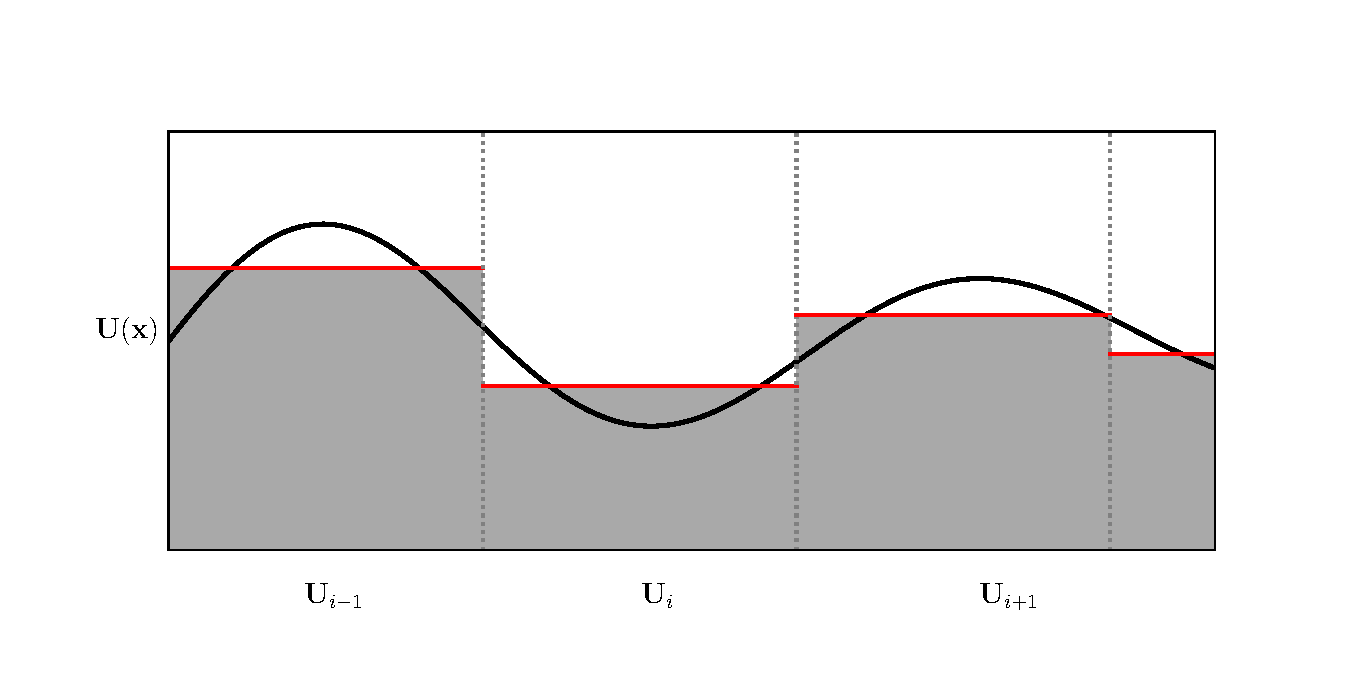
\includegraphics[width=\textwidth]{./figures/piecewise_const.pdf}%
\caption{
A piecewise constant representation of continuous data among cells.
\label{fig:piecewise-constant}
}
\end{figure}

Having a collection of piecewise constant states, we effectively have to solve
local Riemann problems (Section~\ref{chap:riemann} with data $\U_i$ as $\U_L$
and $\U_{i+1}$ as $\U_R$, centered at the intercell boundary positions
$x_{i+\half}$. The solution of the Riemann problem will depend on
$\frac{\bar{x}}{\bar{t}}$, where $\bar{x}$ and $\bar{t}$ are in local
coordinates to the specific Riemann problem under consideration. $\bar{x}$ is
zero at $x_{i+\half}$ and increasingly negative with decreasing $i$. $\bar{t}$
is zero at the current timestep.


Now suppose that we have solved the Riemann problem at the position
$x_{i+\half}$ with left state $\U_L = \U_i$ and right state $\U_R = \U_{i+1}$.
Then, as time evolves, how will the state at $x_{i+\half}$ change?

Recall that the elementary waves travel along characteristics, and that the
characteristics are straight lines on the $x-t$ - diagram (see
Fig.~\ref{fig:riemann-solution}. Then the state at $x_{i+\half}$, which is
where the dividing line between the two initial states is, will be given by the
solution of the Riemann problem at the position $\bar{x} = 0$, and will remain
the same for all $\bar{t} > 0$. (This is assuming there is nothing else that
might disturb the current situation.)


Using that fact, it can be derived that in 1D (see \cite{toro}):

\begin{align}
\U^{n+1}_i &=
	\U^n_i + \frac{\Delta t}{\Delta x}
	\left[
		\F(\U_{i-\half}) - \F(\U_{i+\half})
	\right]
\label{eq:godunov-discretized}
\\
&=
	\U^n_i + \frac{\Delta t}{\Delta x}
	\left[
		\F_{i-\half} - \F_{i+\half}
	\right]
\nonumber
\end{align}

where $\U_{i-\half}$ and $\U_{i+\half}$, $\F_{i-\half}$ and $\F_{i+\half}$ are
the solutions to the Riemann problems at $x_{i-\half}$ and $x_{i+\half}$,
respectively.


It is noteworthy that this is an exact solution to a piecewise constant initial
state.




Lastly, we need to limit the time step size, i.e. find the maximal permissible
time step size. For example, we mustn't allow for a wave to be able to travel
further than one cell length between two timesteps, otherwise we get bogus
results. Recall that we assumed that the state at $x_{i+\half}$ doesn't
change after $\bar{t} > 0$.
This is only satisfied if the wave doesn't reach the boundary of the
neighbouring cell.

This time step restriction is imposed by the CFL condition:

\begin{align}
\Delta t_{max} \leq \frac{C_{cfl} \Delta x}{|S_{max}^n|}
\label{eq:godunov-cfl}
\end{align}


where $S_{max}^n$ is the highest wave propagation speed at the current time,
and $C_{cfl} \in [0, 1($ is the Courant number.


However, this is not the most practical way of doing things.
In 2D, using dimensional splitting (Section~\ref{chap:dimensional-splitting}),
we'd have to first solve everything in one direction to find the wave speeds,
then advance the time step of the sweep, then do the other sweep and hope that
the maximal wave velocity won't be greater than the one of the previous sweep.
Or re-do the first sweep iteratively until we get decent time steps.

Instead, we use the estimate

\begin{align}
	S^n_{max} = \max\{ |v_i^n| + a_i^n \}
\end{align}

This is not always accurate, and the wave speed can be underestimated, leading
to instabilities. To combat this, we just need to choose a lower $C_{cfl}$.
Toro recommends to use $C_{cfl} < 0.8 - 0.9$.













%===================================================================
\subsubsection{Algorithm Details}\label{chap:godunov-details}
%===================================================================

Each cell contains 4 gas states:

\begin{enumerate}
\item The primitive state $\mathbf{W} = (\rho, \V, p)$ of the gas as \code{prim}
\item The flux of the primitive state $\F(\mathbf{W})$ as \code{pflux}
\item The conserved state $\U = (\rho, \rho \V, E)$ of the gas as \code{cons}
\item The flux of the conserved state $\F(\U)$ as \code{cflux}
\end{enumerate}


A flux at position $x_{i+\half, j}$ or $y_{i, j+\half}$ will be stored in the
cell with index $(i, j)$.


We can afford to store $x_{i+\half}$ at cell $i$ because we have at least 1
extra virtual boundary cell which is used to apply boundary conditions, so the
flux at $x_{-\half}$ will be stored in \verb|grid[BC-1]|, where \texttt{BC} is
the number of boundary cells used.
 

\todo{Adapt function name}

We treat the 2D solution using dimensional splitting
(Section~\ref{chap:dimensional-splitting}). Here, we describe the 1D algorithm.

The \verb|solver_step(...)| function does the following for the 1D case:

\begin{itemize}

\item Reset the stored fluxes from the previous timestep to zero.

\item Compute the primitive states for all cells from the updated conserved
states.

\item Impose boundary conditions (Section~\ref{chap:boundary-conditions})

\item Find the maximal permissible timestep by applying the CFL condition
\ref{eq:godunov-cfl}.

\item Compute the fluxes:

\begin{itemize}

\item For every cell pair $(i, i+1)$, solve the Riemann problem
	(Section~\ref{chap:riemann}) to find the flux $\F_{i+\half}$.
\item Store the flux $\F_{i+\half}$ in cell $i$.
\end{itemize}
\item Update the states: Compute $\U^{n+1}$ at this point using
$\U_i^n$, the flux $\F_{i+\half}$ stored in every cell $i$, and the flux
$\F_{i-\half}$ stored in every cell $i-1$ following
Eq.~\ref{eq:godunov-discretized}.
\end{itemize}




